\documentclass[10pt]{beamer}
\usepackage{graphicx}
\usepackage{tikz}
\usepackage{lmodern}
\usepackage{mathtools}
\usepackage{amsmath,bm}
\usepackage{minted}
\usepackage[backend=bibtex]{biblatex}
\usepackage{hyperref}
\usepackage{multirow}

\usetheme{CambridgeUS}
\usecolortheme{seahorse}
\setbeamercovered{dynamic}
\usefonttheme{professionalfonts}
\setbeamertemplate{itemize items}[default]
\setbeamerfont{caption}{size=\footnotesize}
\addbibresource{bibliography.bib}
\setcounter{tocdepth}{2}

\newcommand*{\Scale}[2][4]{\scalebox{#1}{$#2$}}%
\newcommand*{\Resize}[2]{\resizebox{#1}{!}{$#2$}}%
%% Frame Title %%%%%%%%%%%%%%%%%%%%%%%%%%%%%%%%%%%
%\AtBeginSection[]
%{
%  \begin{frame}
%    \frametitle{Table of Contents}
%    \tableofcontents[currentsection]
%  \end{frame}
%}
%%%%%%%%%%%%%%%%%%%%%%%%%%%%%%%%%%%%%%%%%%%%%%%%%%

\begin{document}

\title[Compact finite differences on GPUs]
{A novel approach to evaluating 
compact finite differences 
and similar tridiagonal schemes on GPU-accelerated clusters}


\author[Ashwin Srinath]{
        Ashwin Srinath\\
        Department of Mechanical Engineering\\
        \today \newline \\
        \textbf{Committee members:} \\
        Dr. Gang Li \\
        Dr. Richard S. Miller \\
    Dr. Lonny Thompson}
\date{}
\titlepage

\begin{frame}{Overview}
    \tableofcontents
\end{frame}


\section{Motivation}

\begin{frame}
\frametitle{Direct Numerical Simulation}

An approach for numerically solving
the Navier-Stokes equations

\begin{itemize}
\item Extremely fine computational grids
\item High-order accurate numerical schemes
    \begin{itemize}
    \item Compact finite difference schemes
    \item Spectral methods
    \end{itemize}
\item High computational cost
    \begin{itemize}
    \item Feasible only for simple flows
    \item Parallelism almost always required
    \end{itemize}
\end{itemize}
\end{frame}

\begin{frame}
\frametitle{Compact finite difference schemes}
\centering
\includegraphics[width=200px]{img/discretize-function.eps}
\begin{itemize}
\item High-order accurate finite difference schemes
for evaluating spatial derivatives
\item Able to resolve high wavenumber fluctuations
\item Currently used in our research code
    and in CFDNS (Los Alamos National Lab)
\item {General form of compact schemes:
\begin{align*}
\begin{split}
f_i^{\prime} + \alpha(f^{\prime}_{i-1} + f^{\prime}_{i+1}) + \
\beta(f^{\prime}_{i-2} + f^{\prime}_{i+2}) + \hdots  = \
a\frac{f_{i+1} - f_{i-1}}{dx} + \\
b\frac{f_{i+2} - f_{i-2}}{dx} + \
c\frac{f_{i+3} - f_{i-3}}{dx} + \
    \hdots
\end{split}
\end{align*}}
\end{itemize}
\end{frame}

\begin{frame}[t]
\frametitle{Compact finite difference schemes}
\footnotesize
\begin{itemize}
\item Compact schemes require solution of \emph{banded}
    linear systems (tridiagonal, pentadiagonal)
\item E.g., {$O(dx^4)$ Pad\'{e} scheme yields:
\footnotesize
\begin{equation*}
\begin{bmatrix}
     1&2\\
     1/4&1&1/4\\
     &1/4&1&1/4\\
     &&1/4&1&1/4\\
     &&&1/4&1&1/4\\
     &&&&&\ddots\\
     &&&&&&\ddots\\
     &&&&&&&\ddots\\
     &&&&&&&2&1
  \end{bmatrix}
  \boxed{
  \begin{bmatrix}
      f^{\prime}_1 \\
      f^{\prime}_2 \\
      f^{\prime}_3 \\
      \vdots \\
      \vdots \\
      \vdots \\
      \vdots \\
      f^{\prime}_{n-1} \\
      f^{\prime}_n
   \end{bmatrix}
   }
 =
 \begin{bmatrix}
     \frac{-5f_1 + 4f_2 + f_3}{2dx}\\
     \frac{3(f_{3} - f_{1})}{4dx}\\
     \frac{3(f_{4} - f_{2})}{4dx}\\
     \vdots\\
     \vdots\\
     \vdots\\
     \vdots\\
     \frac{3(f_{n} - f_{n-2})}{4dx}\\
     \frac{5f_{n} - 4f_{n-1} - f_{n-2}}{2dx}
  \end{bmatrix}
\end{equation*}}
\item Solution yields the derivative at
    all points $i=1, 2, \hdots n$ simultaneously
\item Tridiagonal schemes generally sufficient
\item Expensive, difficult to parallelize
\end{itemize}
\end{frame}

\begin{frame}
\frametitle{Objectives}
\begin{itemize}
\item Exploratory work for exploiting GPUs
    in current research code
    \begin{itemize}
    \item important step for our group: Palmetto cluster
    currently has 598 GPUs (and counting)
    \end{itemize}
\item Develop an efficient GPU tridiagonal solver
    for compact finite difference evaluation
\item Parallelize the compact finite difference evaluation---current
    research code uses a sequential approach
\end{itemize}
\end{frame}

\begin{frame}
\frametitle{Thesis contributions}
\begin{itemize}
\item Present a novel algorithm for
    the tridiagonal systems arising in
    compact finite differences
    and similar numerical schemes
\item Present a strategy for evaluating compact
    finite differences on GPU-accelerated clusters
\item Show enhanced performance relative to existing
    tridiagonal algorithms (discussed below)
\item Contributions for both single GPU
    and multiple GPUs
\end{itemize}
\end{frame}



\subsection{Graphics processing units}

\begin{frame}[t]
\frametitle{Introduction}
\pause
\begin{columns}[T]
\begin{column}{0.4\textwidth}
\begin{itemize}
    \item <2-> Highly multi-threaded processor
        \begin{itemize}
            \item NVIDIA Tesla K20 accelerator: 2496 cores
        \end{itemize}
    \item <3-> Spectacular performance for
        \emph{compute-intensive, data-parallel} operations
    \item <4-> Not suited for general-purpose computation
    \item <5-> Requires careful redesign of algorithms,
        substantial code changes, and tuning efforts
\end{itemize}
\end{column}
\begin{column}{0.6\textwidth}
\visible<2-> {
    \vspace{2cm}
    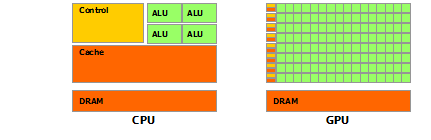
\includegraphics[width=180px]
    {img/device-comparison.png}
}
\end{column}
\end{columns}
\end{frame}

\begin{frame}
\frametitle{Programming GPUs}
\pause
Scientific applications use GPUs at various levels:
\begin{itemize}
    \item Low-level
        \begin{itemize}
            \item CUDA
            \item OpenCL
        \end{itemize}
    \item High-level
        \begin{itemize}[<+->]
            \item OpenACC compiler directives
            \item Drop-in support for scientific libraries such as Intel MKL, BLAS
        \end{itemize}
    \item Transparent
        \begin{itemize}[<+->]
            \item MATLAB: over 200 functions
            \item Software packages: Abaqus, ANSYS (Mechanical/Fluent)
        \end{itemize}
\end{itemize}
\end{frame}

\begin{frame}
\frametitle{CUDA programming model}
\pause
\begin{columns}
\begin{column}{0.5\textwidth}
\textbf{Kernels}
\begin{itemize}[<+->]
    \item Special pieces of code that execute on the GPU
    \item In Fortran: subroutines; in C: functions
    \item Executed concurrently by several GPU threads
\end{itemize}
\textbf{Threads}
\begin{itemize}[<+->]
    \item Threads organized into a grid of blocks
    \item Kernels launched with specified grid size
        (number of blocks) and block size (threads per block)
    \item Grid and blocks can be 2-D or 3-D for convenience
\end{itemize}
\end{column}
\begin{column}{0.5\textwidth}
    \only<5-6>{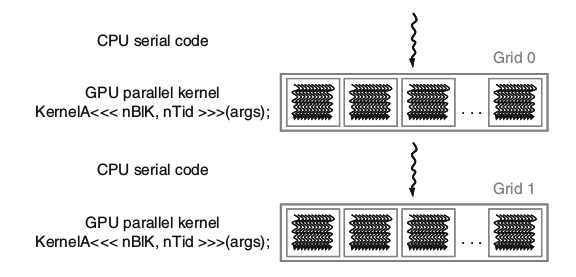
\includegraphics[width=150px]{img/program-structure.png}}
    \only<7>{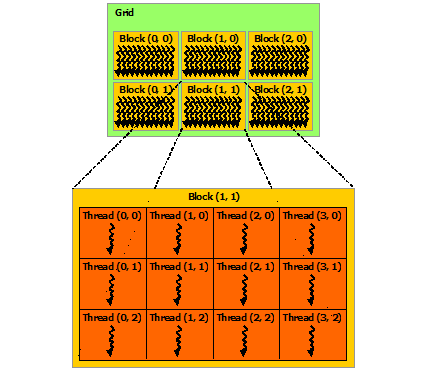
\includegraphics[width=150px]{img/grid-of-thread-blocks.png}}
\end{column}
\end{columns}
\end{frame}

\begin{frame}
\frametitle{GPU architecture and memory model}
\pause
\begin{columns}
\begin{column}{0.5\textwidth}
\begin{itemize}[<+->]
    \item GPU viewed as a collection of \emph{streaming microprocessors} (SMs)
    \item When kernel is launched, each block gets assigned to an SM
    \item Threads within a block execute concurrently
    \item SM may execute several blocks concurrently
\end{itemize}
\end{column}
\begin{column}{0.5\textwidth}
    \visible<3->{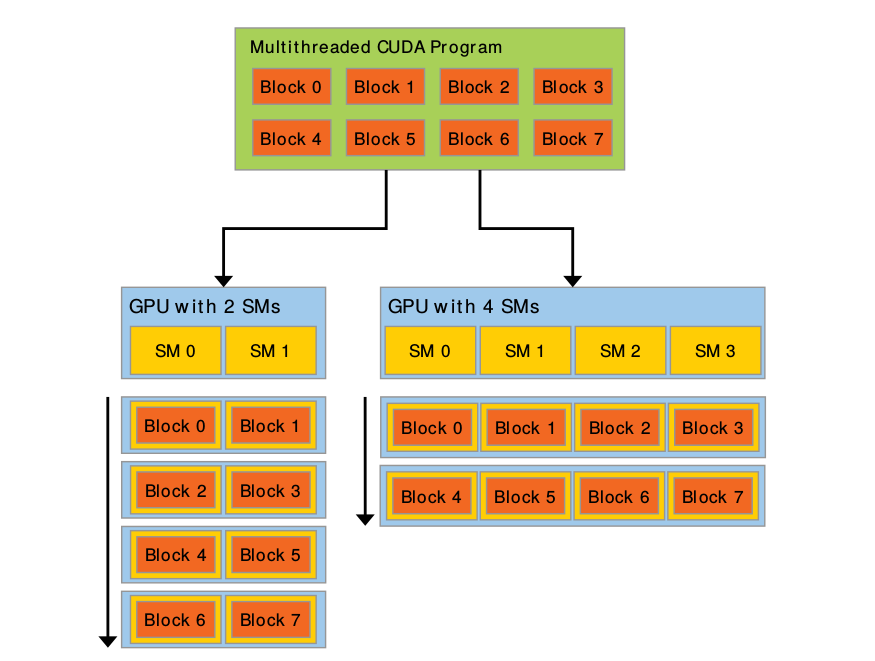
\includegraphics[width=150px]{img/gpu-scaling.png}}
\end{column}
\end{columns}
\end{frame}

\begin{frame}
\frametitle{GPU architecture and memory model}
\pause
\begin{columns}
\begin{column}{0.5\textwidth}
\begin{itemize}
    \item Global memory{
        \begin{itemize}
            \item large but slow (~5 GB for Tesla K20)
            \item all threads can access
            \item persists between kernel launches
        \end{itemize}}
    \item Shared memory{
        \begin{itemize}
            \item small but fast (~48 KiB per SM)
            \item local to threads within a block
            \item explicitly managed cache
        \end{itemize}}
    \item Registers{
        \begin{itemize}
            \item limited (65536 per SM)
            \item local to individual threads
            \item fastest
        \end{itemize}}
\end{itemize}
\end{column}
\begin{column}{0.5\textwidth}
    \visible<2->{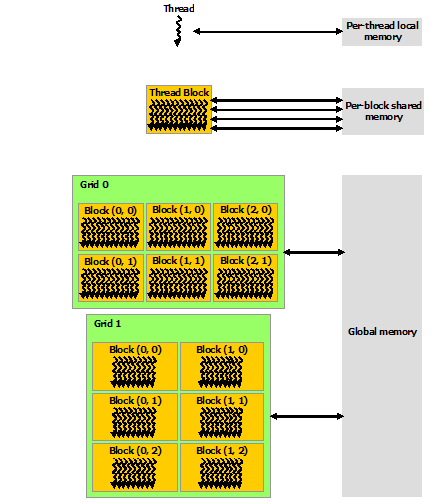
\includegraphics[width=150px]{img/memory-hierarchy.png}}
\end{column}
\end{columns}
\end{frame}


\section{Developing a GPU tridiagonal solver}

\begin{frame}
\frametitle{Requirements of tridiagonal solver}
\begin{columns}
\begin{column}{0.5\textwidth}
\begin{itemize}
\item For a 1-D grid, solution gives the derivative
    at all points simultaneously
\item For 2-D and 3-D grids,
    must solve many independent tridiagonal systems
\item Systems have the same tridiagonal coefficients,
    different right hand sides
\item Need a tridiagonal solver that solves
    a given system for several right hand sides
\item For 2-D problems $n \sim N_{rhs}$;
    for 3-D problems $n << N_{rhs}$
\end{itemize}
\end{column}
\begin{column}{0.5\textwidth}
    \hspace{1cm}
    \includegraphics[width=120px]{img/grid-lines.eps}
\end{column}
\end{columns}
\end{frame}

\begin{frame}
\frametitle{Thomas algorithm}
\begin{itemize}
\item Derived from Gaussian elimination
\item Requires $2n$ steps and $4n$ storage
\item The most efficient sequential algorithm
\item What about parallelization/GPUs?
    \begin{itemize}
        \item inherently sequential
        \item use multiple threads to solve
            individual tridiagonal systems
            (Sakharnykh et al.)
    \end{itemize}
\end{itemize}
\end{frame}

\begin{frame}
\frametitle{Issues in GPU implementation}
\begin{columns}
\begin{column}{0.5\textwidth}
\begin{itemize}
    \item Uncoalesced memory accesses
    \item Needs data rearrangement to coalesce accesses
    \item Does not expose enough parallelism
    \item $2n$ steps - can do better on GPU
    \item A case in which \emph{algorithm choice
        significantly impacts GPU performance}
\end{itemize}
\end{column}
\begin{column}{0.5\textwidth}
    \includegraphics[width=120px]{img/pThomas.eps}
\end{column}
\end{columns}
\end{frame}

\begin{frame}
\frametitle{Tridiagonal solvers for the GPU}
\begin{itemize}
\item Zhang et al. (2010) describe the implementation
    of three algorithms for tridiagonal systems on GPUs
    \begin{itemize}
        \item Cyclic reduction
        \item Parallel cyclic reduction
        \item Recursive doubling
    \end{itemize}
\item \textbf{Step efficient}: trade more work per step for \emph{fewer steps}
\item Exhibit \emph{fine-grained} parallelism - more suited to GPU
\item Subsequent efforts based on CR and PCR primarily
\end{itemize}
\end{frame}

\begin{frame}
\frametitle{Cyclic reduction}
\begin{columns}
\begin{column}{0.5\textwidth}
\begin{itemize}
\item Buzbee and Goleb (1970)
\item \textbf{Forward reduction} ($log_2(n)-1$ steps):
    \begin{itemize}
    \item Eliminate odd-indexed equations at each step
    \item Two-by-two system is left
    \end{itemize}
\item \textbf{Backward substitution} ($log_2(n)-1$ steps):
    \begin{itemize}
    \item Solve for odd-indexed equations using even-indexed values
    \end{itemize}
\item Best case ($n$ parallel threads): requires $2log_2(n)-1$ steps
\end{itemize}
\end{column}
\begin{column}{0.5\textwidth}
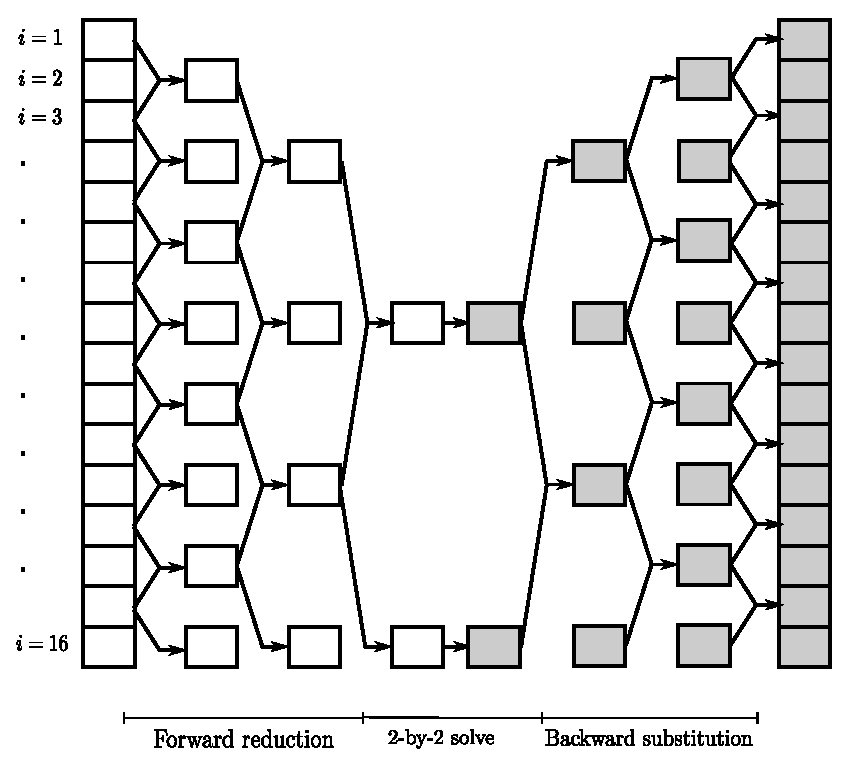
\includegraphics[width=150px]{img/cyclic-reduction.eps}
\end{column}
\end{columns}
\end{frame}

\begin{frame}
\frametitle{Cyclic reduction}
\begin{columns}
\begin{column}{0.5\textwidth}
\begin{itemize}
\item $17n$ operations,
    compared to $8n$ in Thomas algorithm
\item But exhibits more parallelism:
\begin{itemize}
    \item Individual systems can be solved independently
    \item Individual equations can be computed independently
\end{itemize}
\item Equations updated in place: $4n$ storage (same as Thomas algorithm)
\item Synchronization between threads required at each step
\end{itemize}
\end{column}
\begin{column}{0.5\textwidth}
\centering
Forward reduction

(diagonals $a$, $b$, $c$ and RHS $d$)
\scalebox{0.8}{
\vbox{
\begin{align*} 
    k_1 &= \frac{a_i}{b_{i-1}}, k_2 = \frac{c_i}{b_{i+1}} \\
    a^{\prime}_i &= -a_{i-1}k_1 \\
    b^{\prime}_i &= b_i - c_{i-1}k_1 - a_{i+1}k_2 \\
    c^{\prime}_i &= -c_{i+1}k_2 \\
    d^{\prime}_i &= d_i - d_{i-1}k_1  - d_{i+1}k_2 \\
\end{align*}}}

\centering
Backward substitution
\scalebox{0.8}{
\vbox{
\begin{align*}
x_i &= \frac{d^{\prime}_i - a^{\prime}_ix_{i-1} - \
    c^{\prime}_ix_{i+1}}{b^{\prime}_i}
\end{align*}}}
\end{column}
\end{columns}
\end{frame}

\begin{frame}
\frametitle{Issues in GPU implementation}
\footnotesize
\begin{columns}
\begin{column}{0.5\textwidth}
\begin{itemize}
    \item Strided memory access:
        stride increases by a factor of 2 at each step
        (decreases during backward substitution)
    \item \textbf{Solution}: use \emph{shared memory} (cache)
    \item Thread activity decreases during forward
        reduction and increases during backward substitution
    \item \textbf{Solution}: schedule threads for each step
        \begin{itemize}
            \footnotesize
            \item conflicts with shared memory usage
        \end{itemize}
    \item Shared memory \emph{bank conflicts}
        due to power-of-2 strides; reduced GPU occupancy
    \item We provide both implementations:
        global memory \emph{and} shared memory
\end{itemize}
\end{column}
\begin{column}{0.5\textwidth}
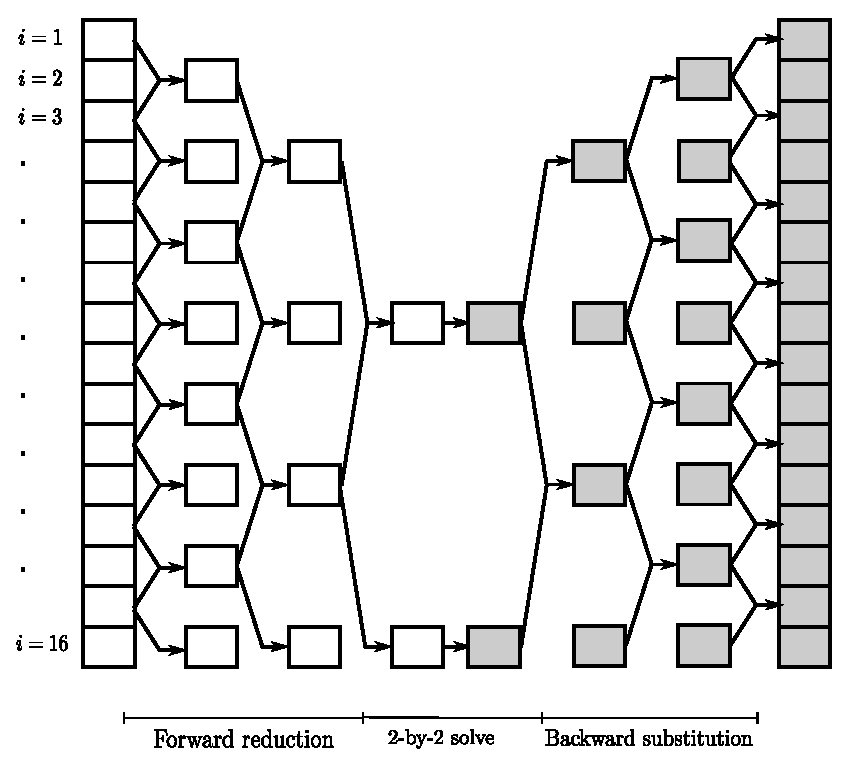
\includegraphics[width=150px]{img/cyclic-reduction.eps}
\end{column}
\end{columns}
\end{frame}

\begin{frame}
\frametitle{Efforts for improving performance}
\begin{itemize}
    \item Zhang et al.: hybrid CR+PCR solver
    \item G{\"o}ddeke et al.: separate even and odd indexed
        coefficients
    \item Davidson et al.: register packing
    \item Esfahanian et al.: global memory with data rearrangement
\end{itemize}
\end{frame}

\begin{frame}
\frametitle{A novel approach}
\begin{columns}
\begin{column}{0.5\textwidth}
\begin{itemize}
\item Solving system with same matrix and different RHS
\item Computing $a^\prime$, $b^\prime$ and $c^\prime$
    for each system and at every time step - \textbf{redundant}
\item Storing coefficients (similar to LU) - \textbf{expensive}
\item Approach: exploit the simple matrix structure
\end{itemize}
\end{column}
\begin{column}{0.5\textwidth}
\centering
Forward reduction
\scalebox{0.8}{
\vbox{
\begin{align*} 
    k_1 &= \frac{a_i}{b_{i-1}}, k_2 = \frac{c_i}{b_{i+1}} \\
    a^{\prime}_i &= -a_{i-1}k_1 \\
    b^{\prime}_i &= b_i - c_{i-1}k_1 - a_{i+1}k_2 \\
    c^{\prime}_i &= -c_{i+1}k_2 \\
    d^{\prime}_i &= d_i - d_{i-1}k_1  - d_{i+1}k_2 \\
\end{align*}}}
\end{column}
\end{columns}
\end{frame}

\begin{frame}
\frametitle{A novel approach}
\begin{columns}
\begin{column}{0.5\textwidth}
\begin{itemize}
\item Diagonals are nearly constant (\emph{near-Toeplitz tridiagonal})
\item Symmetry broken by boundary conditions
\item Near-Toeplitz trdiagonal matrices occur in other numerical schemes
\begin{itemize}
    \item Alternating direct implicit methods
    \item Line relaxation methods
    \item Poisson solvers
    \item One-dimensional ODEs and PDEs
\end{itemize}
\item Can be stored compactly compared to general tridiagonal systems
\end{itemize}
\end{column}
\begin{column}{0.5\textwidth}
\centering
\scalebox{0.6}{%
\vbox{
\begin{equation*}
\begin{bmatrix}
     1&2\\
     1/4&1&1/4\\
     &1/4&1&1/4\\
     &&1/4&1&1/4\\
     &&&1/4&1&1/4\\
     &&&&&\ddots\\
     &&&&&&\ddots\\
     &&&&&&&\ddots\\
     &&&&&&&2&1
  \end{bmatrix}
\end{equation*}}}
\end{column}
\end{columns}
\end{frame}

\begin{frame}
\frametitle{General approach}
\begin{columns}
\begin{column}{0.5\textwidth}
\begin{itemize}
\item Each forward reduction step reduces
    a matrix of size $n$ to $n/2$
\item {First reduction step: substitute:
    \scalebox{0.8}{
    \vbox{
    \begin{align*}
        a_2 &= a_3 = a_4 = \hdots &\equiv a_0 \\
        b_2 &= b_3 = b_4 = \hdots &\equiv b_0 \\
        c_2 &= c_3 = c_4 = \hdots &\equiv c_0
    \end{align*}}}}
\item \textbf{The resulting reduced system is also near-Toeplitz}
\item Each subsequent forward reduction step produces a near-Toeplitz
    tridiagonal system
\begin{itemize}
    \item can be stored compactly
    \item no need to compute for each RHS/time step
\end{itemize}
\end{itemize}
\end{column}
\begin{column}{0.5\textwidth}
\centering
Forward reduction
\scalebox{0.8}{
\vbox{
\begin{align*} 
    k_1 &= \frac{a_i}{b_{i-1}}, k_2 = \frac{c_i}{b_{i+1}} \\
    a^{\prime}_i &= -a_{i-1}k_1 \\
    b^{\prime}_i &= b_i - c_{i-1}k_1 - a_{i+1}k_2 \\
    c^{\prime}_i &= -c_{i+1}k_2 \\
    d^{\prime}_i &= d_i - d_{i-1}k_1  - d_{i+1}k_2 \\
\end{align*}}}
\end{column}
\end{columns}
\end{frame}

\begin{frame}
Cyclic reduction reduced to:

\vspace{1cm}

\textbf{Forward reduction}

\hspace{3.85cm} \sout{$k_1 = \frac{a_i}{b_{i-1}}, k_2 = \frac{c_i}{b_{i+1}}$}

\hspace{3.85cm} \sout{$a^{\prime}_i = -a_{i-1}k_1$}

\hspace{3.85cm} \sout{$b^{\prime}_i = b_i - c_{i-1}k_1 - a_{i+1}k_2$}

\hspace{3.85cm} \sout{$c^{\prime}_i = -c_{i+1}k_2$} 
\begin{align*}
d^{\prime}_i = d_i - d_{i-1}k_1^{m}  - d_{i+1}k_2^{m}
\end{align*}

\textbf{Backward substitution}
\begin{align*}
x_i = \frac{d^{\prime}_i - a^mx_{i-1} - \
    c^{m}x_{i+1}}{b^m}
\end{align*}

where $k_1^m$, $k_2^m$, $a^m$, $b^m$ and $c^m$ are the precomputed
coefficients for $i>1$ at the step $m$.
\end{frame}



\section{Application to compact finite differences}

\begin{frame}
\frametitle{Application to compact finite difference schemes}
\begin{itemize}
\item Compact finite difference evaluation involves two steps:
\begin{enumerate}
\item Evaluation of the right hand sides
\begin{itemize}
    \item easily performed on the GPU
\end{itemize}
\item Solving the tridiagonal systems for all the grid lines
\end{enumerate}
\item Current efforts:
\begin{itemize}
    \item Tutkun et al. (2012)
    \item Esfahanian et al. (2014)
\end{itemize}
\item Typical DNS problems too large to fit on a single GPU
\item Need a strategy for multiple GPUs
\end{itemize}
\end{frame}

\begin{frame}
\frametitle{Parallelization strategy: multiple GPUs on a single node}
\begin{columns}
\begin{column}{0.5\textwidth}
\begin{itemize}
\item Method used by Sakharnykh et al.
\item Decompose domain into \emph{subdomains};
    each GPU assigned a subdomain
\item Single subdomain used along derivative direction
\item No coordination between GPUs required
\item For other coordinate directions,
    transpose the data (physically or logically)
\end{itemize}
\end{column}
\begin{column}{0.5\textwidth}
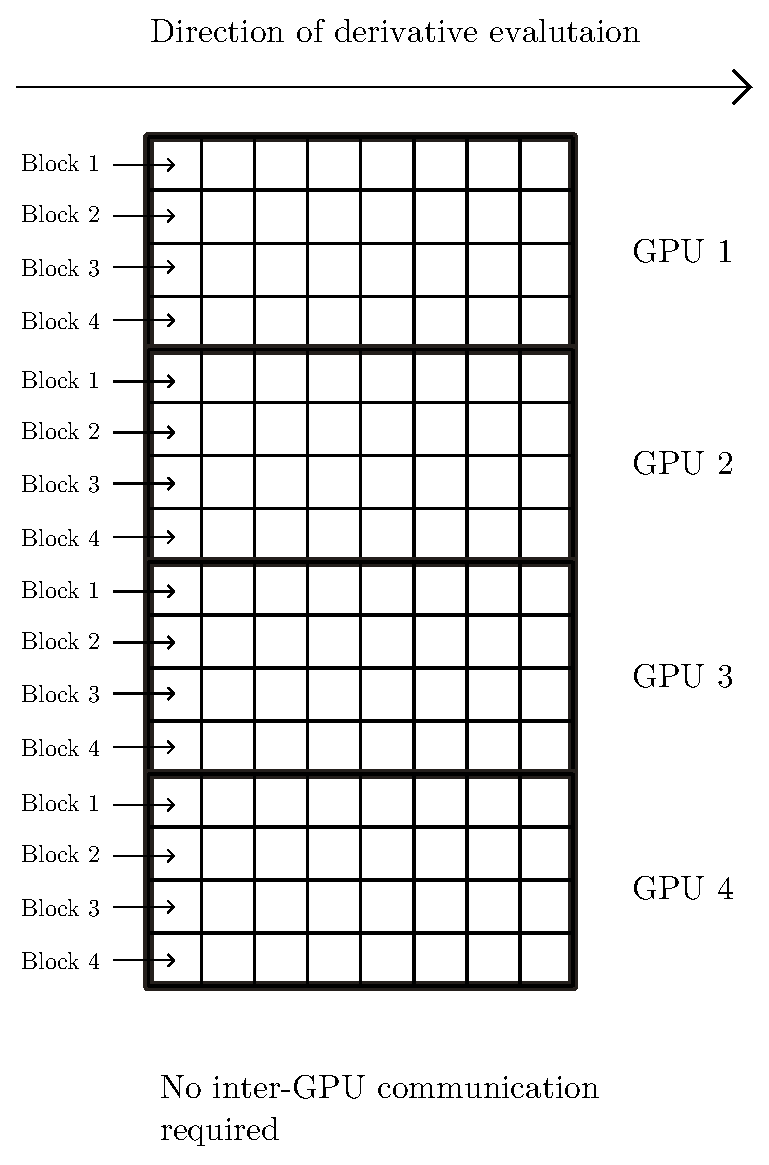
\includegraphics[width=100px]{img/compact-shared-gpu.eps}
\end{column}
\end{columns}
\end{frame}

\begin{frame}
\frametitle{Parallelization strategy: multiple GPUs on distinct nodes}
\begin{columns}
\begin{column}{0.5\textwidth}
\begin{itemize}
\item Single subdomain used along derivative direction
\item No coordination between GPUs required
\item \textbf{Physical} global transpose required
\item Subdomains can become impractically slender
\item Scalable approach needs a distributed tridiagonal solver
\end{itemize}
\end{column}
\begin{column}{0.5\textwidth}
    \only<1>{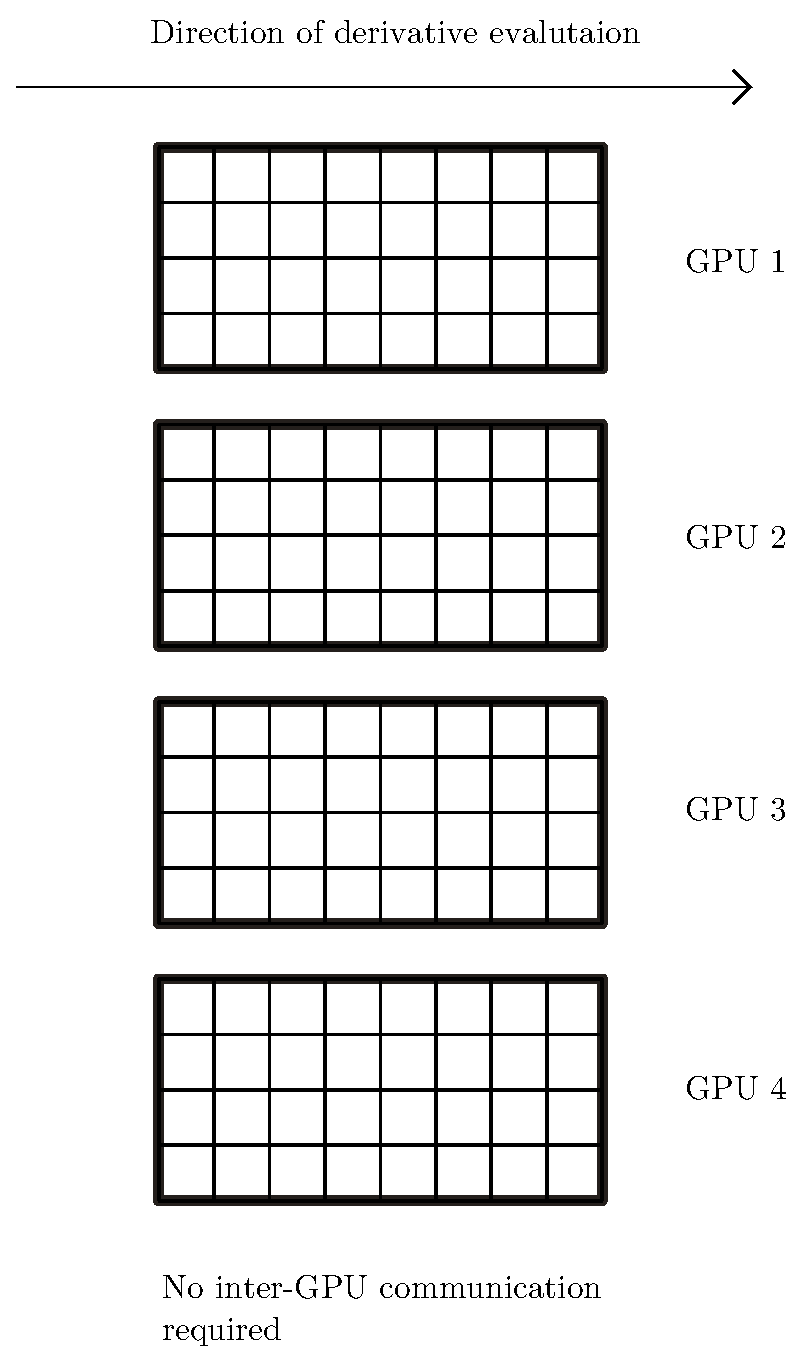
\includegraphics[width=100px]{img/compact-distributed-restricted.eps}}
    \only<2>{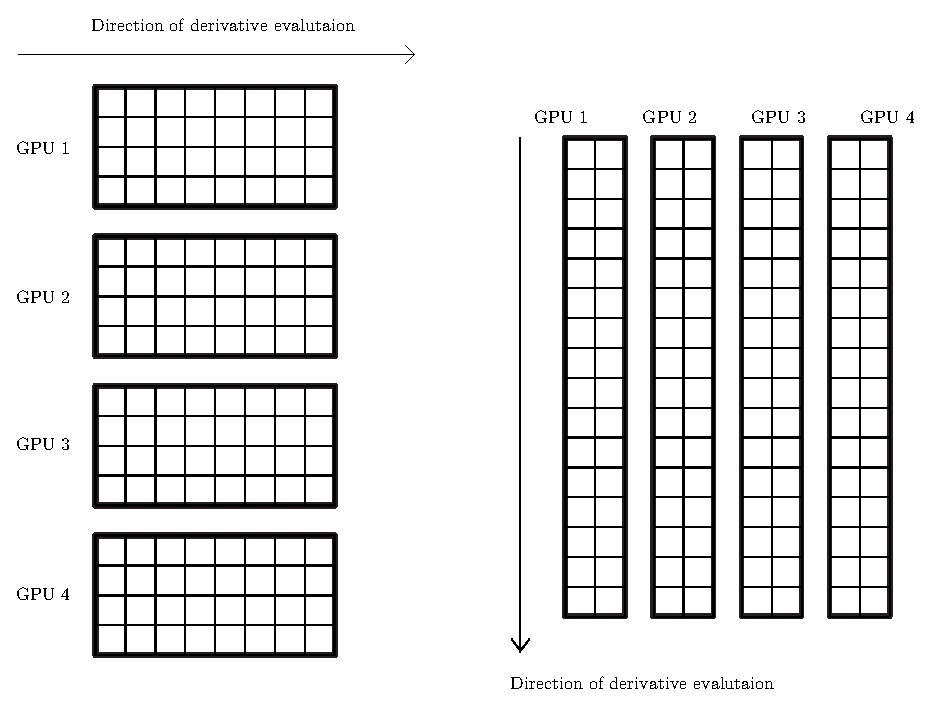
\includegraphics[width=150px]{img/compact-restricted-transpose.eps}}
    \only<3>{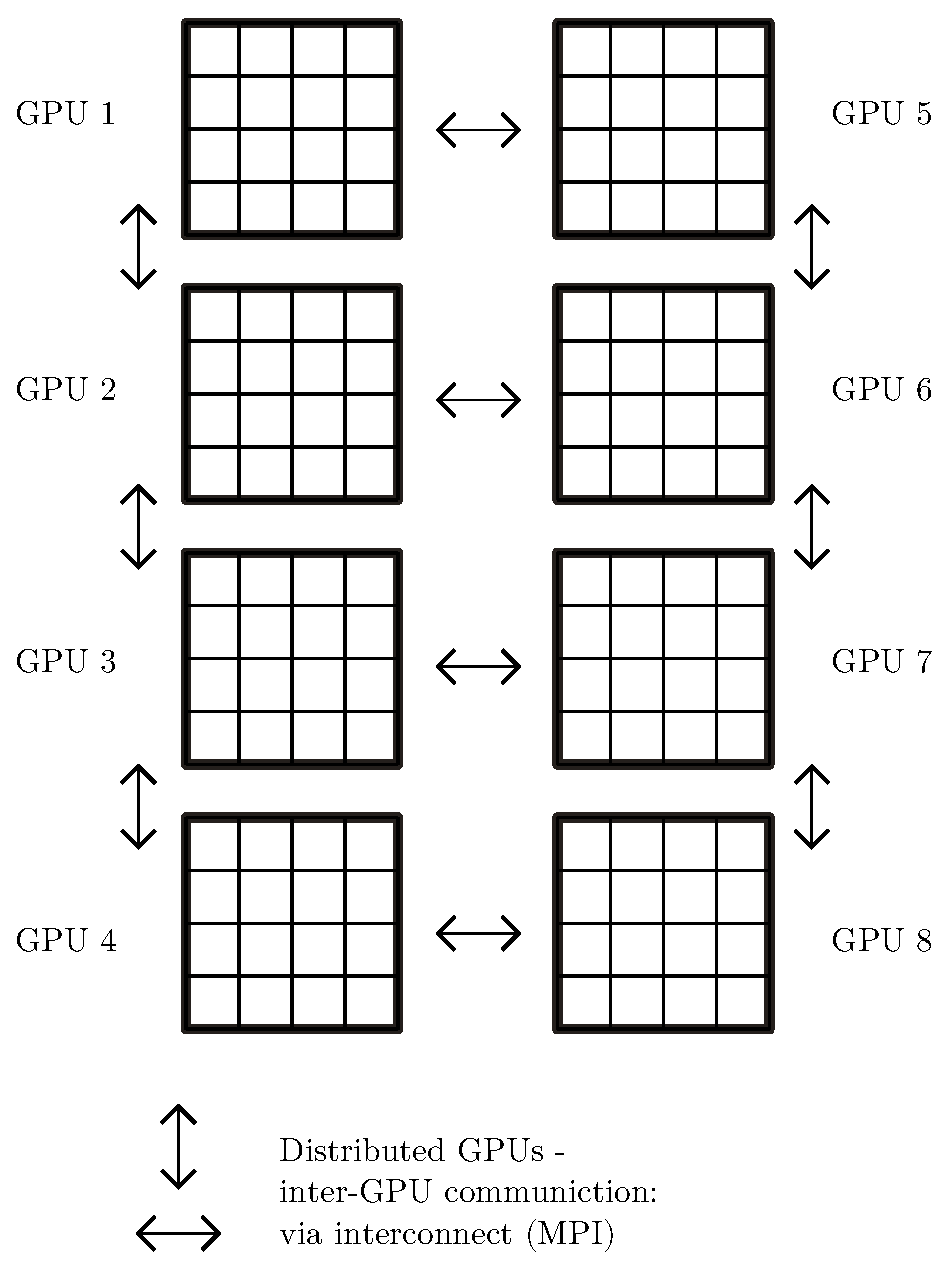
\includegraphics[width=120px]{img/compact-distributed-all.eps}}
\end{column}
\end{columns}
\end{frame}

\begin{frame}
\frametitle{Distributed tridiagonal solver}

Solving a tridiagonal system of size
$mP$, split among $P$ processes (Mattor et al., 1995):

\footnotesize
\begin{columns}
\begin{column}{0.5\textwidth}
\begin{enumerate}
\item Each process solves the local systems:
    \begin{align*}
        A^px_r^{p} &= r_p \\
        A^pu^p &= \{-a_1^p, 0, 0, 0, \hdots\} \\
        A^pl^p &= \{0, 0, 0 \hdots, -c_m^p\}
    \end{align*}
\item Construct and assemble a ``reduced'' system
    of the form:
    \scalebox{0.6}{
        \vbox{
    \begin{align*}
     \begin{bmatrix}
l^1_m & -1 \\
-1    & u^2_1 & l^2_1 \\
  & u^2_m & l^2_m & -1 \\
  &       & -1    & u^3_1 & l^3_1 \\
  &       &       & u^3_m & l^3_m  & -1 \\
  &       &       &       & \ddots & \ddots & \ddots \\
  &       &       &       &        & -1     & u^P_1
\end{bmatrix}
\begin{bmatrix}
\beta^1 \\
\alpha^2 \\
\beta^2 \\
\alpha^3 \\
\beta^3 \\
\vdots \\
\alpha^P
\end{bmatrix}
=
\begin{bmatrix}
x_{r,m}^1 \\
x_{r,1}^2 \\
x_{r,m}^2 \\
x_{r,1}^3 \\
x_{r,m}^3 \\
\vdots \\
x_{r,1}^P \\
\end{bmatrix}  
        \end{align*}}}
\item Local part of solution given by:
\begin{align*}
x^p = x_r^p + \
    \alpha^p u^p + \beta^p l^p
\end{align*}
\end{enumerate}
\end{column}
\begin{column}{0.5\textwidth}
\centering
\includegraphics[width=120px]{img/dividing-tridiagonal.eps}
\end{column}
\end{columns}
\end{frame}

\begin{frame}
\frametitle{Compact finite difference on multi-GPU system}
\footnotesize
\begin{columns}
\begin{column}{0.5\textwidth}
\begin{enumerate}
\item Computing RHS for all local grid points - \textbf{requires communication}
\begin{itemize}
    \footnotesize
    \item halo swaps with neighbouring GPUs
    \item pointwise stencil
\end{itemize}
\item Solving local tridiagonal systems - no communication
\item Assembling and solving reduced tridiagonal systems - \textbf{requires communication}
\begin{itemize}
    \footnotesize
    \item global communication along line of GPUs
    \item produces interleaved tridiagonal sysems - pThomas algorithm
\end{itemize}
\item Summing solutions from steps 2 and 3 - no communication
\begin{itemize}
    \footnotesize
    \item pointwise sum
\end{itemize}
\item For other coordinate directions: \emph{local} permutation of data
\end{enumerate}
\end{column}
\begin{column}{0.5\textwidth}
\only<1>{\includegraphics[width=175px]{img/rhs-halos.eps}}
\only<2>{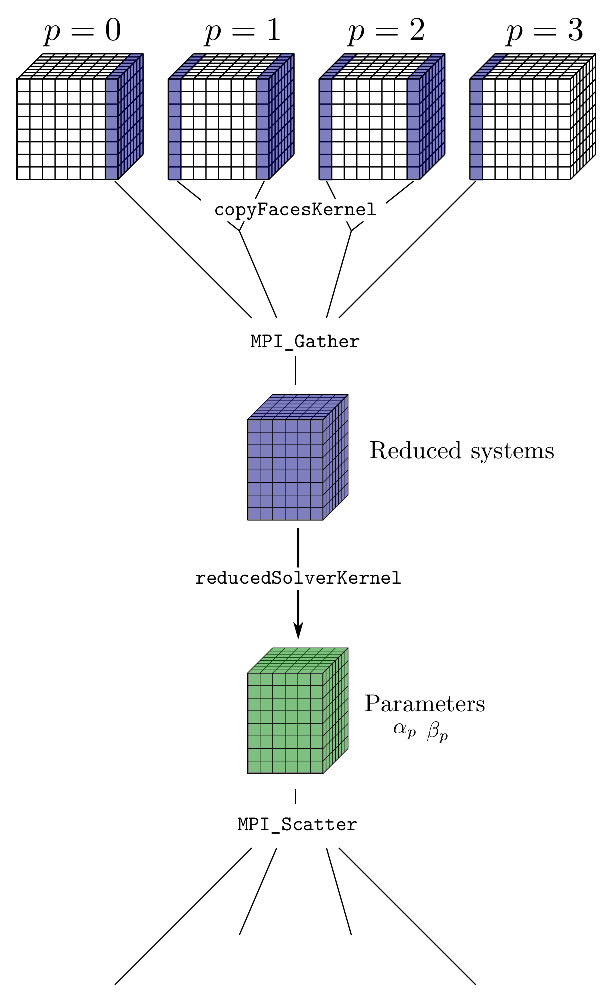
\includegraphics[width=175px]{img/constructing-reduced-system.eps}}
\end{column}
\end{columns}
\end{frame}



\section{Results}

\begin{frame}
\frametitle{Overview of results}
\begin{itemize}
\item Results for tridiagonal solver
\begin{itemize}
    \item Global memory v/s shared memory implementations
    \item Compared against library solvers
        (multicore CPU and GPU)
\end{itemize}
\item Results for compact finite difference application
\begin{itemize}
    \item Profiling results
    \item Scaling results
    \item Comparison with CPU-only approach
\end{itemize}
\end{itemize}
\end{frame}


\begin{frame}
\frametitle{Global memory v/s shared memory implementations}
\begin{columns}
\begin{column}{0.5\textwidth}
\begin{itemize}
\item For 2-D problems, shared memory clearly better
\item For 3-D problems, shared memory speedup
    is smaller
\item Global memory makes better use of
    GPU parallelism in 3-D case
\end{itemize}
\end{column}
\begin{column}{0.5\textwidth}
\centering
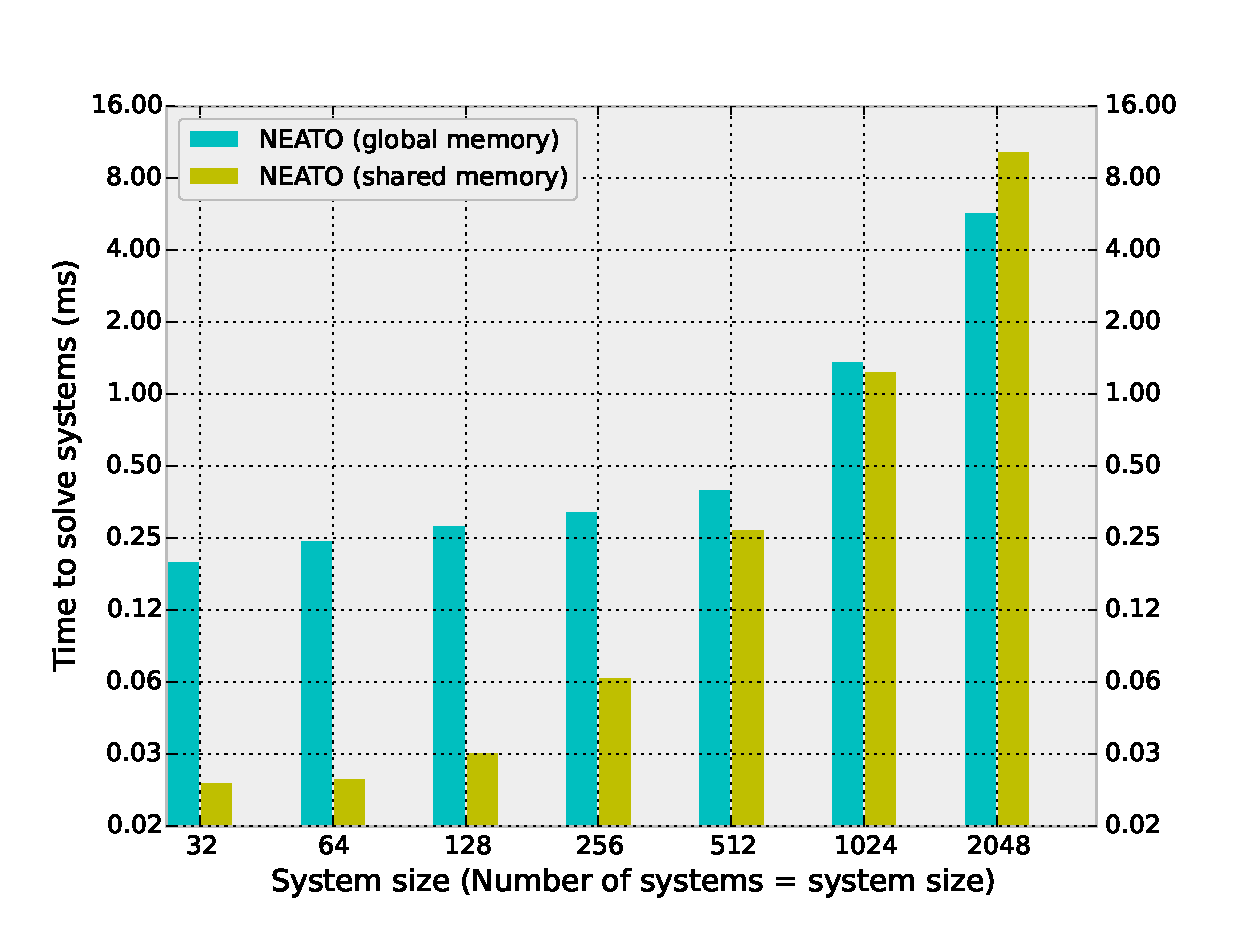
\includegraphics[width=140px]{img/global-vs-shared-2d.eps}

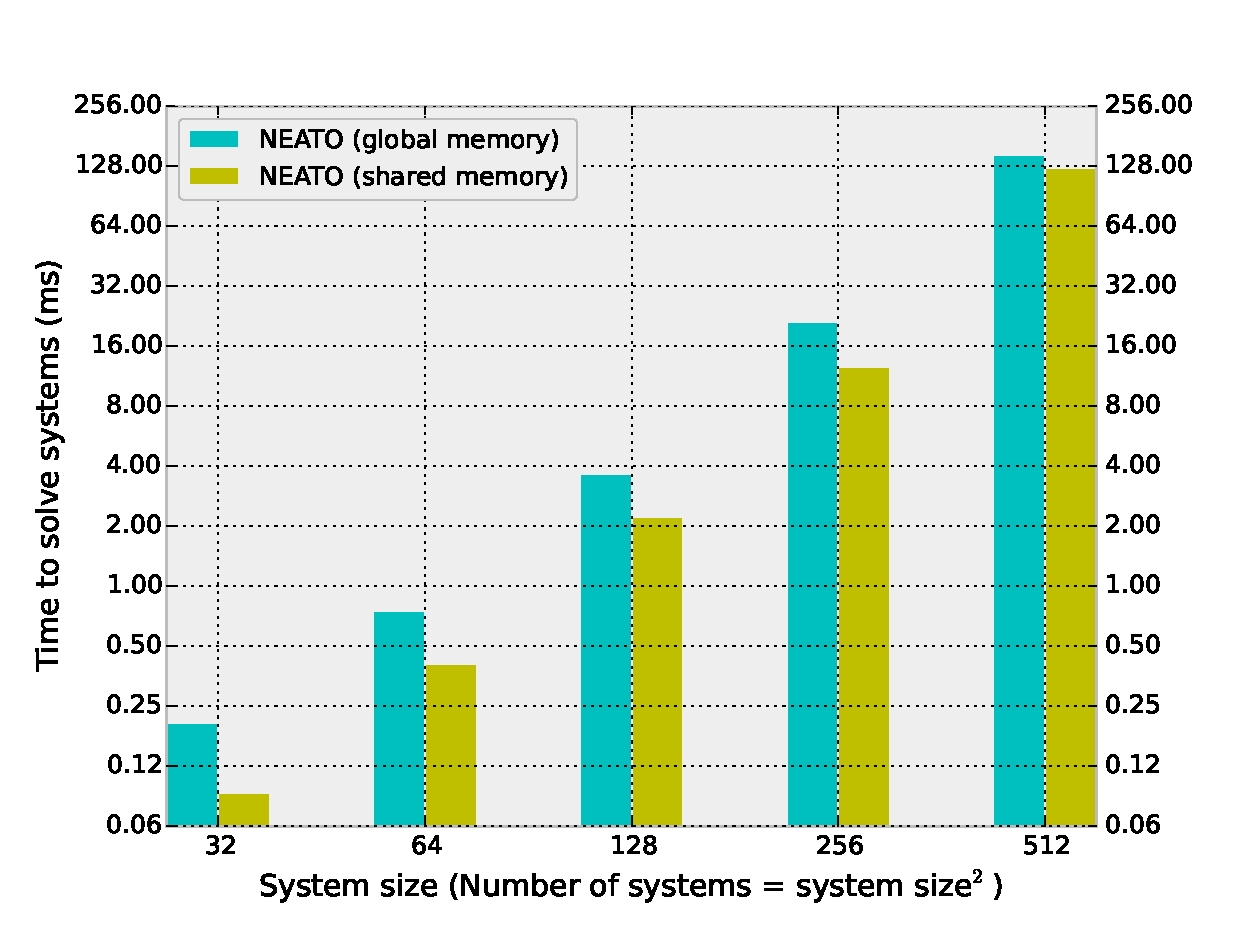
\includegraphics[width=140px]{img/global-vs-shared-3d.eps}
\end{column}
\end{columns}
\end{frame}

\begin{frame}
\frametitle{Comparison with library solvers - timings}
\begin{table}
\resizebox{\textwidth}{!}{%
% Please add the following required packages to your document preamble:
% \usepackage{multirow}
\begin{tabular}{|l|l|l|l|l|l|l|}
\hline
\multirow{2}{*}              & \multirow{2}{*}{}        & \multicolumn{5}{c|}{Time to solve (ms)}                             \\ \cline{3-7}
\centering System size       & Number of systems        & MKL 1 core    & MKL 16 cores & CUSPARSE & NEATO (global) & NEATO (shared) \\ \hline
32                           & 32                       & 0.045         & 0.05         & 0.273    & 0.201          & 0.024          \\ \hline
64                           & 64                       & 0.048         & 0.249        & 0.271    & 0.247          & 0.025          \\ \hline
128                          & 128                      & 0.089         & 0.145        & 0.271    & 0.284          & 0.032          \\ \hline
256                          & 256                      & 0.263         & 0.202        & 0.305    & 0.326          & 0.066          \\ \hline
512                          & 512                      & 0.959         & 0.299        & 0.629    & 0.403          & 0.272          \\ \hline
1024                         & 1024                     & 3.775         & 0.864        & 1.939    & 1.375          & 1.252          \\ \hline
2048                         & 2048                     & 16.272        & 4.111        & 7.607    & 5.811          & 10.407         \\ \hline
32                           & 1024                     & 0.152         & 0.257        & 0.31     & 0.207          & 0.092          \\ \hline
64                           & 4096                     & 0.879         & 0.403        & 0.556    & 0.751          & 0.409          \\ \hline
128                          & 16384                    & 7.052         & 1.931        & 3.128    & 3.669          & 2.225          \\ \hline
256                          & 65536                    & 63.858        & 17.61        & 28.495   & 21.148         & 12.565         \\ \hline
512                          & 262144                   & 515.792       & 159.394      &          & 145.34         & 125.311        \\ \hline 
\end{tabular}

}
\end{table}
\end{frame}

\begin{frame}
\frametitle{Comparison with library solvers - speedup}
\centering
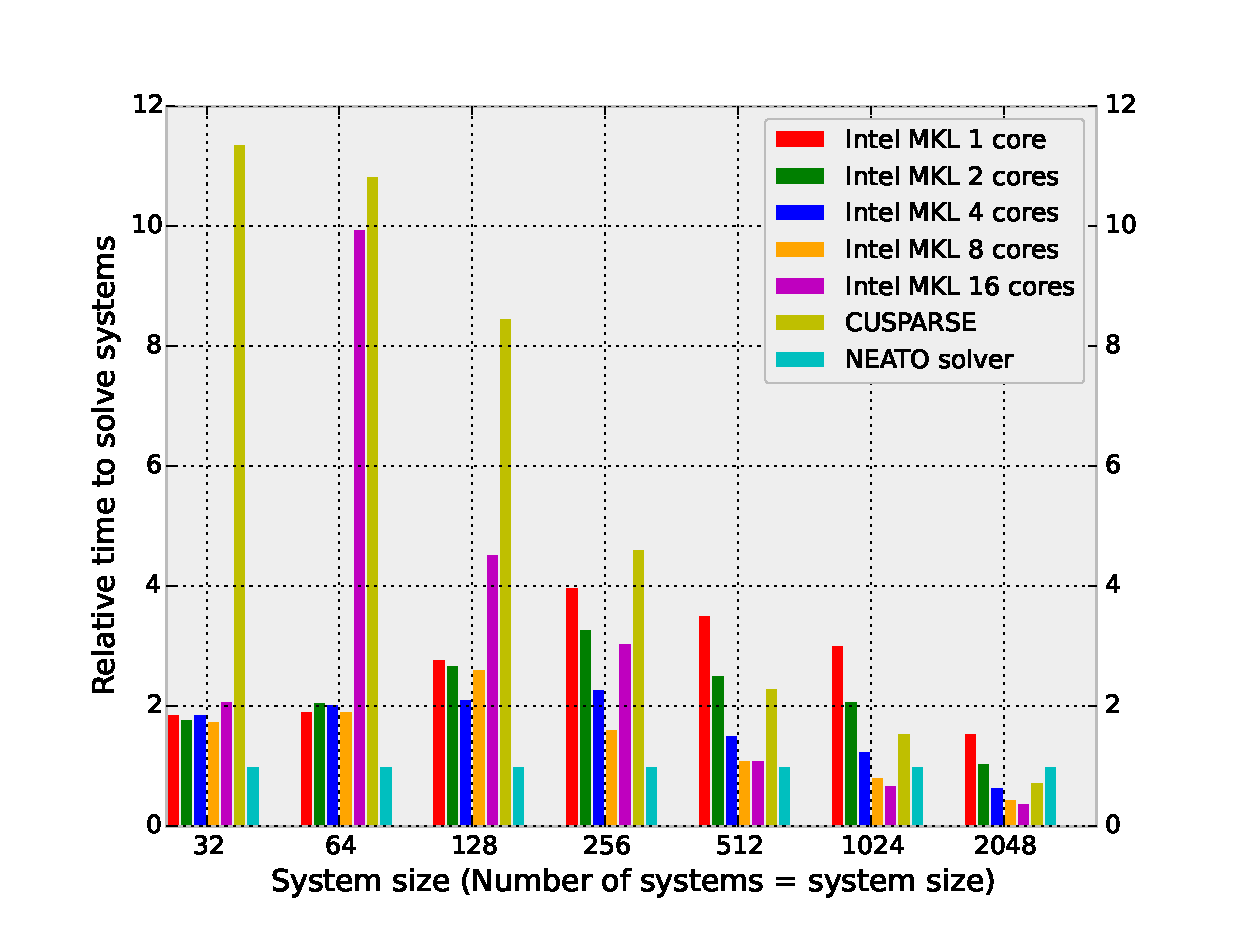
\includegraphics[width=180px]{img/bench-2d.eps}
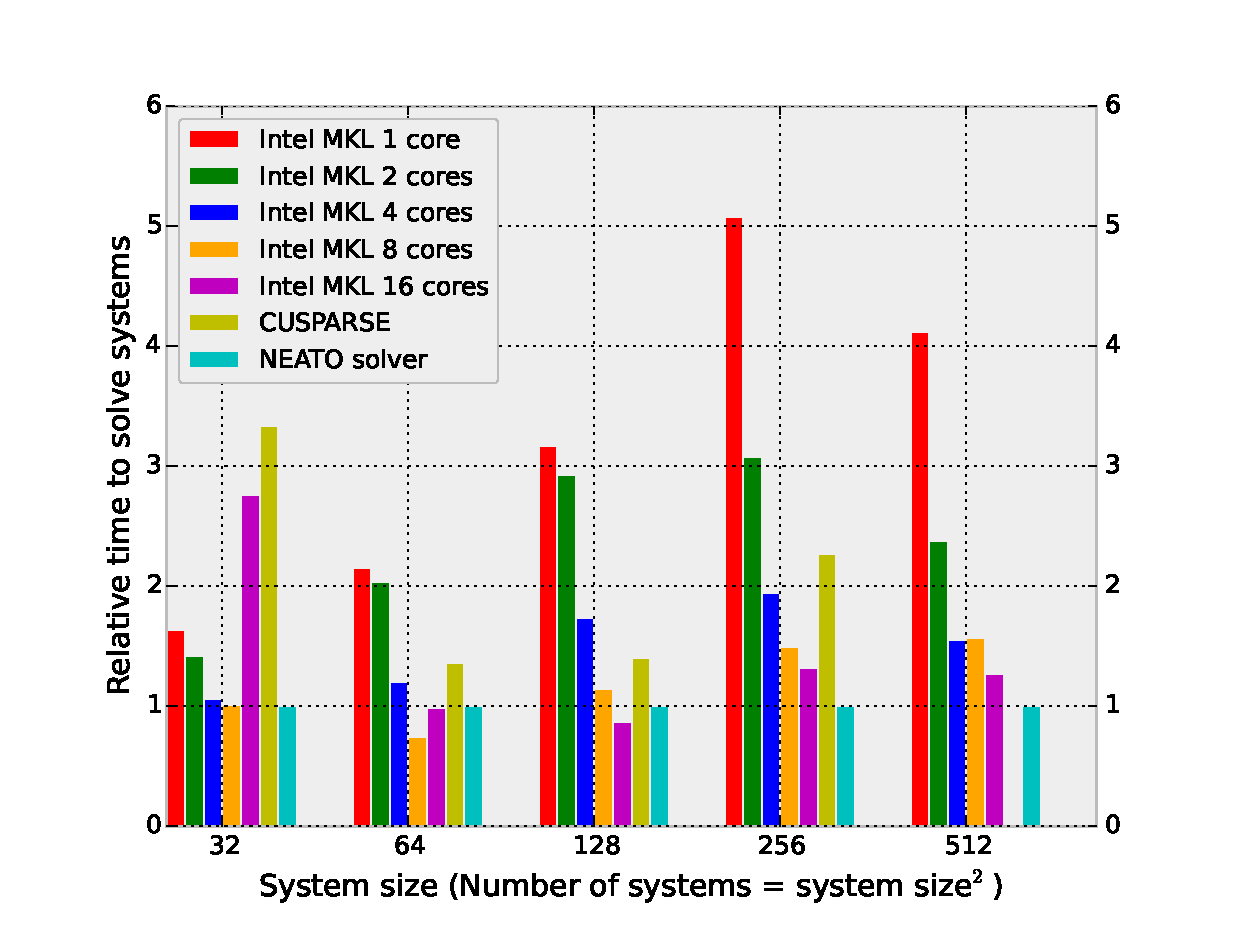
\includegraphics[width=180px]{img/bench-3d.eps}
\begin{table}
\end{table}
\end{frame}

\begin{frame}
\frametitle{Note on speedups}
\begin{itemize}
\item Comparing against 8 CPU cores, speedups in the range 1-2x
\item Solving the tridiagonal systems
    is the \emph{least amenable to efficient parallel solution}
\item Objective is to keep the problem on the GPU
\end{itemize}
\end{frame}

\begin{frame}
\frametitle{Compact finite difference evaluation - profiling}
\begin{columns}
\begin{column}{0.5\textwidth}
\begin{itemize}
    \item Problem sizes: $1024^3$ and $2048^3$ on 64 GPUs
    \item For larger problems, more time spent
        on tridiagonal systems
    \item Significant portion of time spent on
        data permutation
\end{itemize}
\end{column}
\begin{column}{0.5\textwidth}
\centering
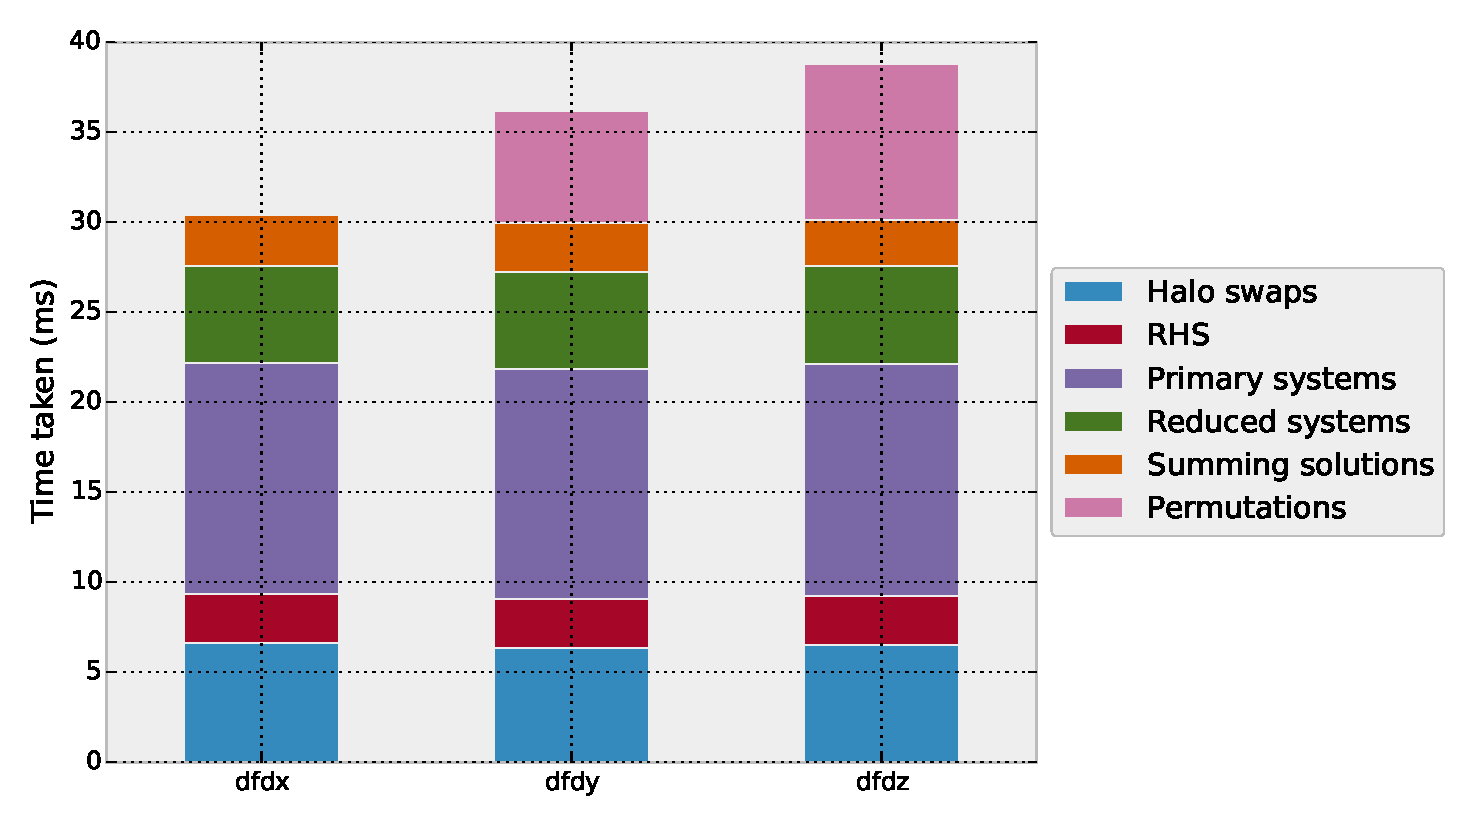
\includegraphics[width=170px]{img/profiling-1024-64.eps}

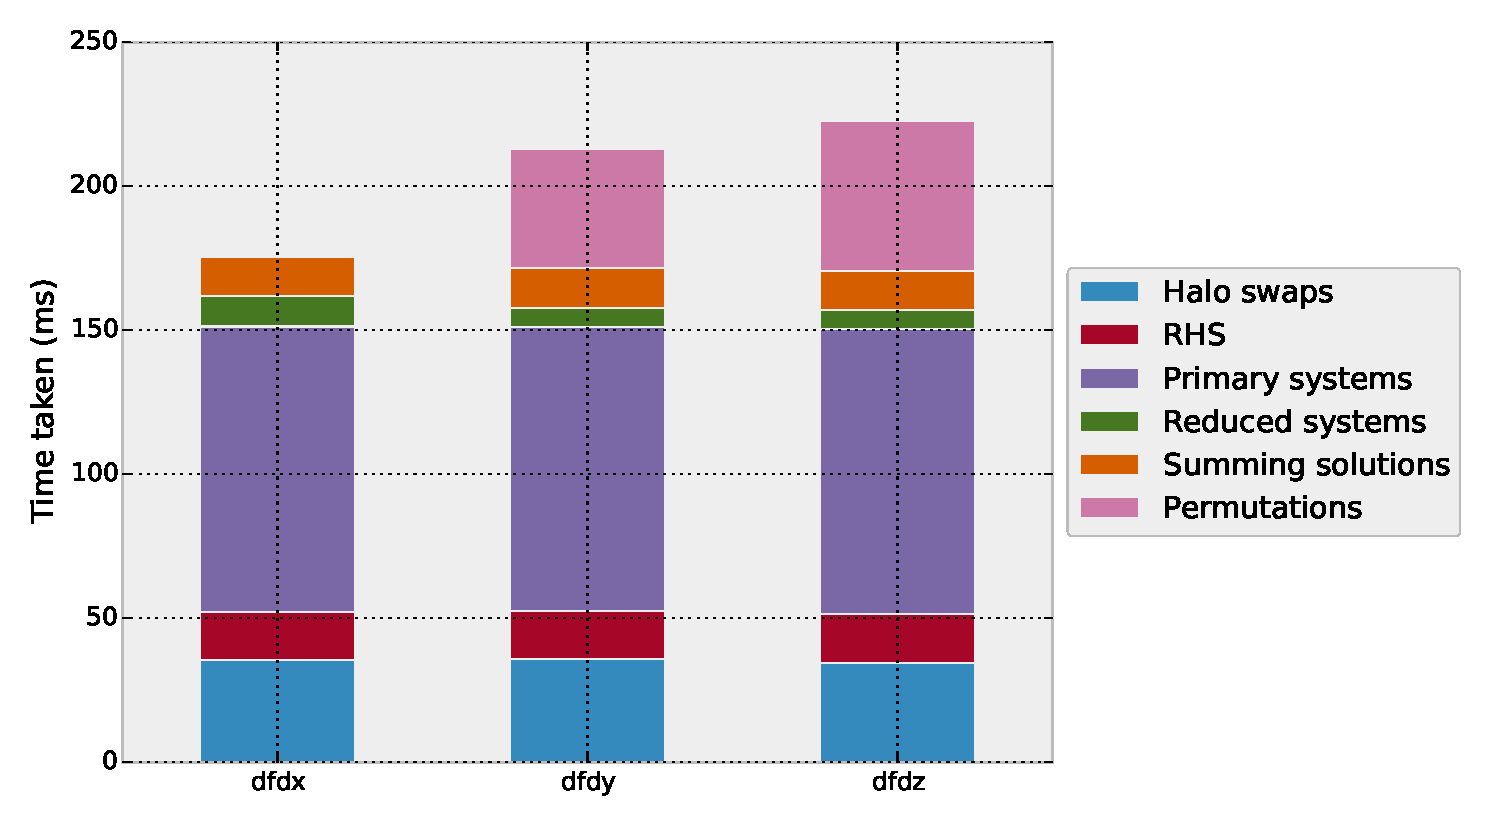
\includegraphics[width=170px]{img/profiling-2048-64.eps}
\end{column}
\end{columns}
\end{frame}

\begin{frame}
\frametitle{Compact finite difference evaluation - strong scaling}
\centering
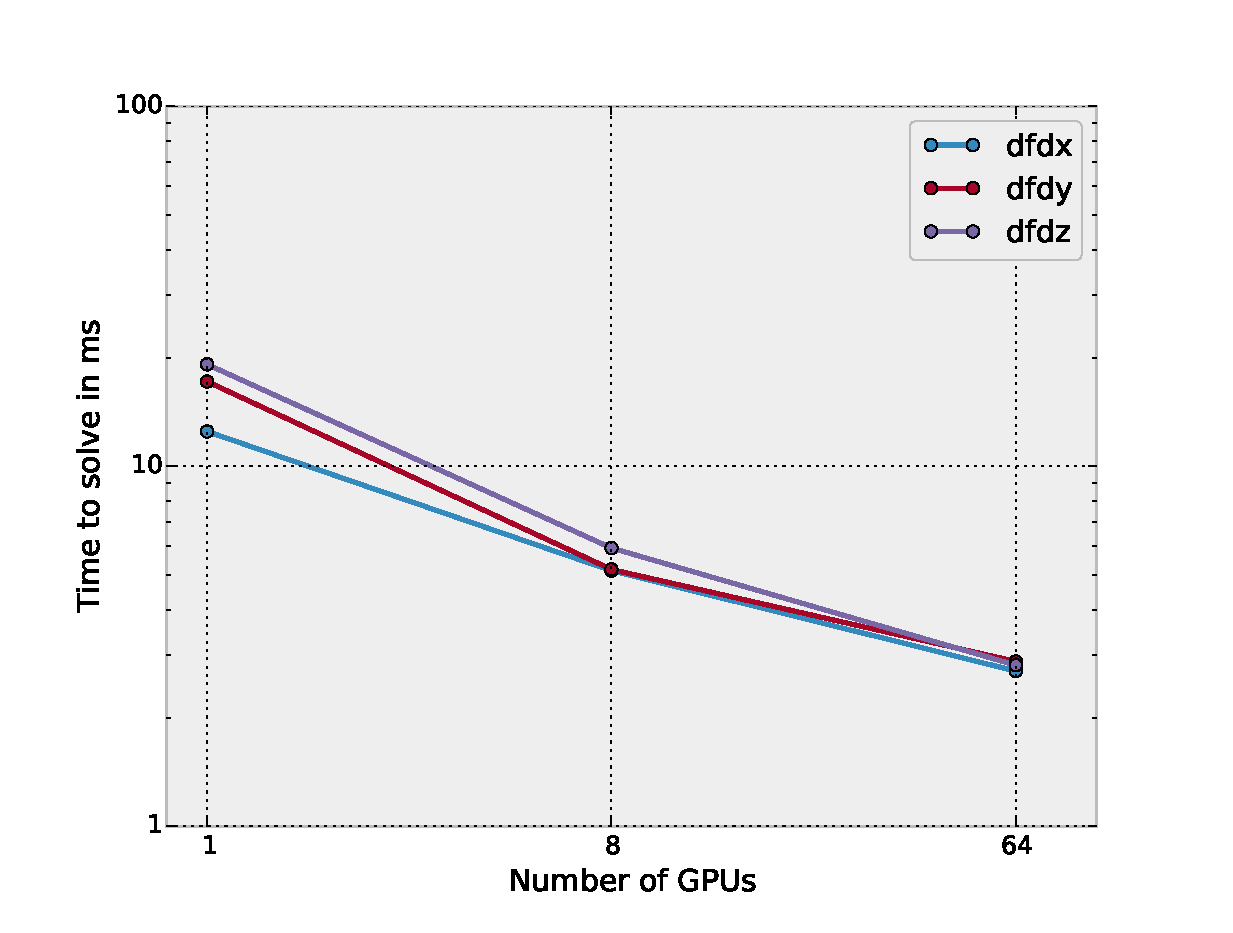
\includegraphics[width=180px]{img/strong-scaling-256.eps}
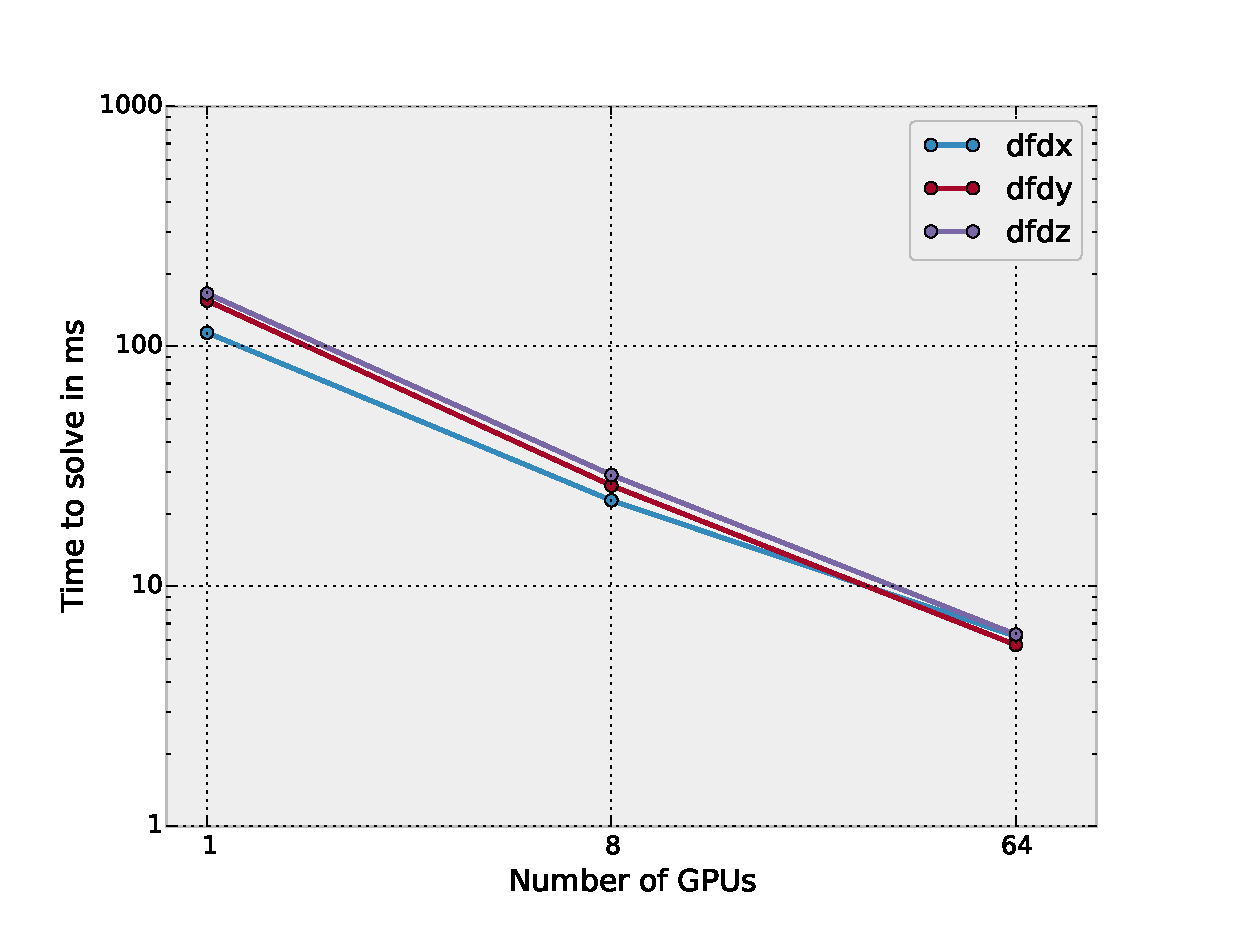
\includegraphics[width=180px]{img/strong-scaling-512.eps}

Problem sizes: $256^3$ and $512^3$
\end{frame}

\begin{frame}
\frametitle{Compact finite difference evaluation - weak scaling}
\centering
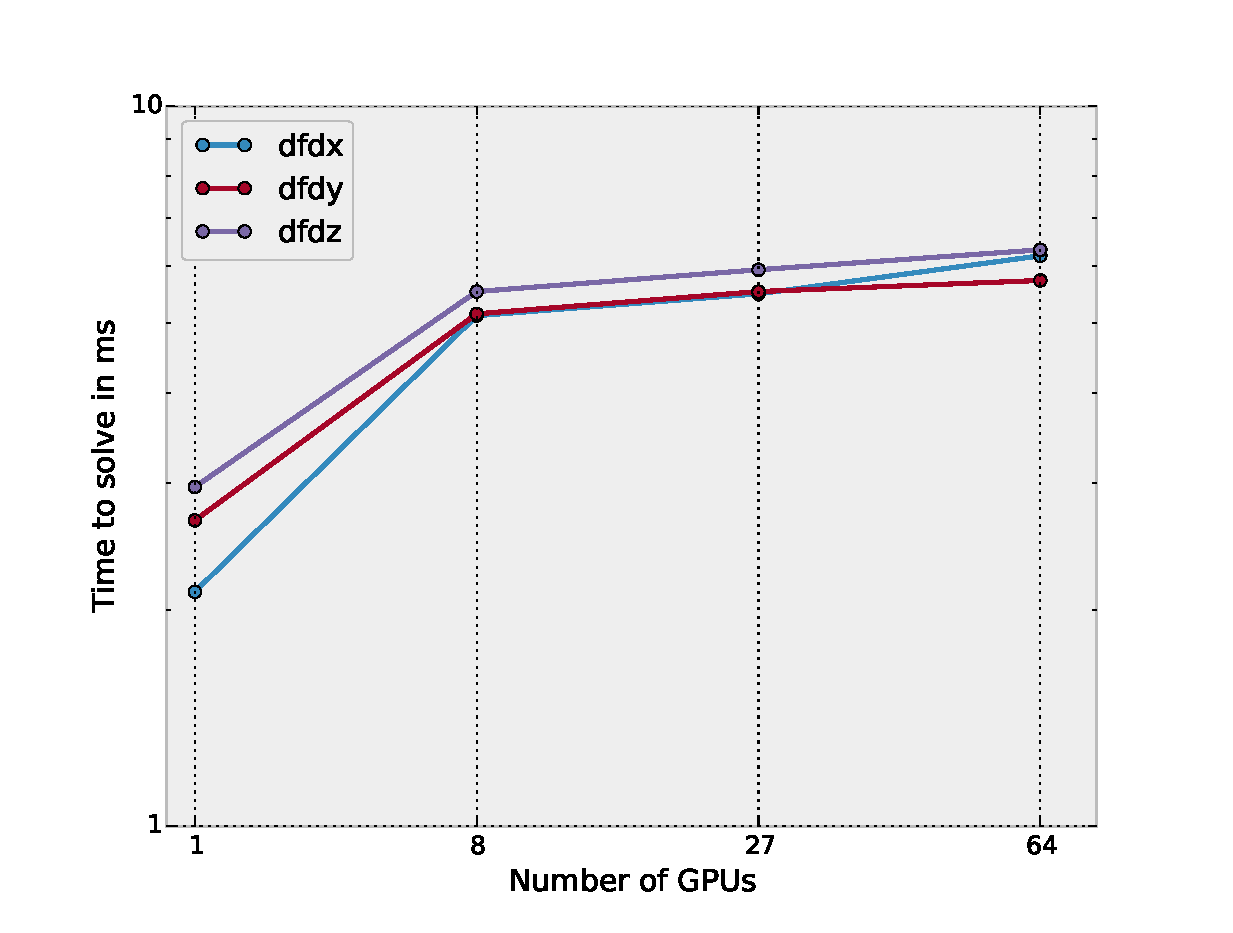
\includegraphics[width=180px]{img/weak-scaling-128.eps}
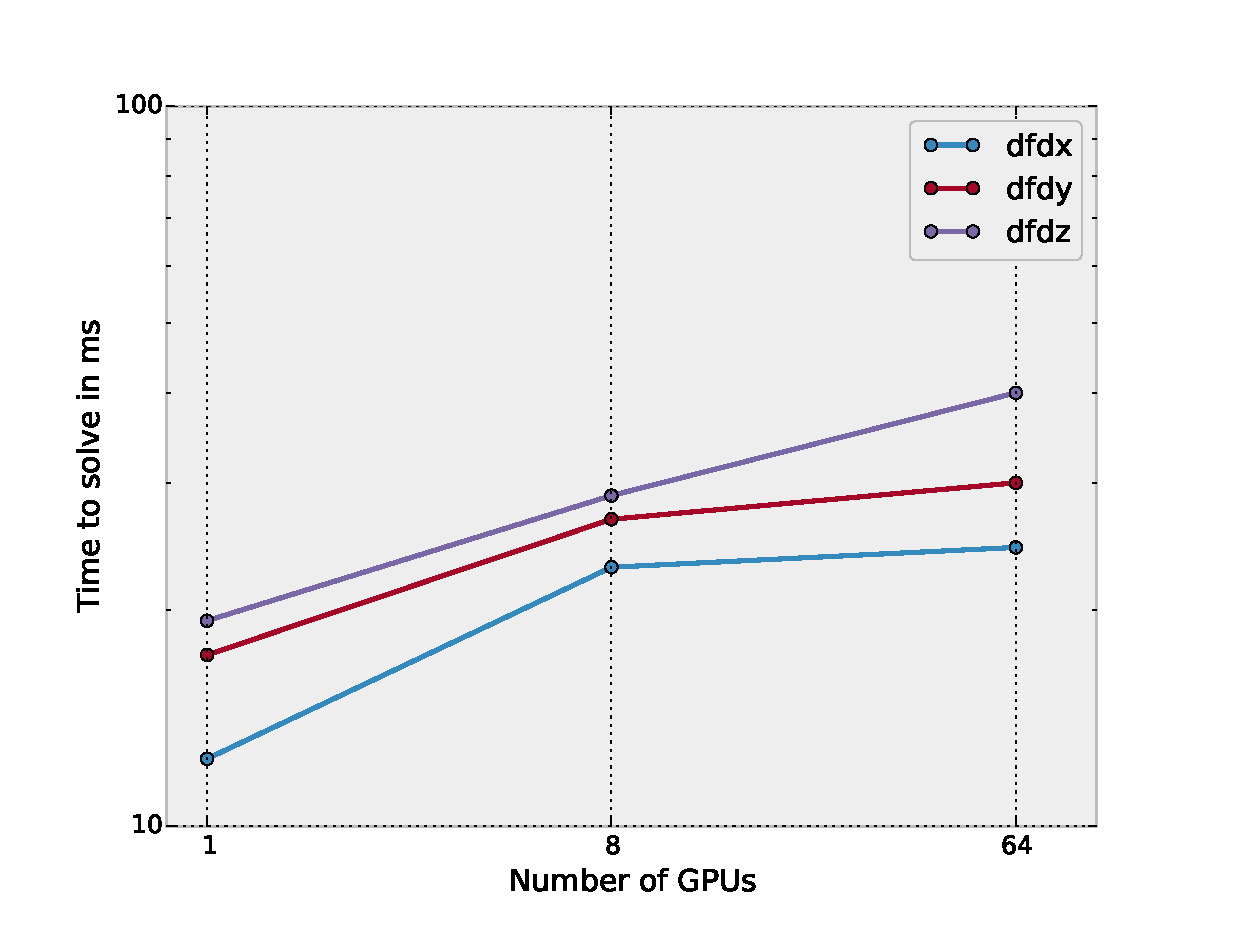
\includegraphics[width=180px]{img/weak-scaling-256.eps}

Problem sizes: $128^3$ and $256^3$ \emph{per process}
\end{frame}

\begin{frame}
\frametitle{Comparison with CPU-only approach}
\begin{columns}
\begin{column}{0.5\textwidth}
\begin{itemize}
\item Reference implementation: approach in CFDNS code
    (Los Alamos National Lab)
\item Maintain a ratio of 8 CPU cores : 1 GPU in comparison
\end{itemize}
\end{column}
\begin{column}{0.5\textwidth}
\centering
\begin{table}
\resizebox{0.75\textwidth}{!}{%
\centering
\begin{tabular}{|l|l|l|l|l|l|l|}
\hline
\multirow{2}{*}{Size} & \multicolumn{3}{c|}{Ref. impl, \#CPU cores} & \multicolumn{3}{c|}{NEATO-based, \#GPUs} \\ \cline{2-7}
         & 8         & 64        & 512      & 1       & 8       & 64      \\ \hline
$256^3$  & 79.5      & 20.8      & 11.1     & 19.9    & 5.17    & 2.79    \\ \hline
$512^3$  & 556.8     & 146.5     & 29.2     & 164.5   & 23.24   & 5.62    \\ \hline
$1024^3$ & 5188      & 1092      & 223.7    & -       & 174.9   & 24.49   \\ \hline
$2048^3$ & -         & -         & 1741     & -       & -       & 297.07  \\ \hline
\end{tabular}

}
\end{table}

\includegraphics[width=140px]{img/compact-refimpl-speedups.eps}
\end{column}
\end{columns}
\end{frame}


\end{document}

